\section{Homology of configuration spaces of surfaces}
\label{sec:HBraidSurf}
We want to study $H_*(\bms)=H_*(\cms)$,
which appears as the homology of the fiber
in the Leray-Serre spectral sequence associated to
\ref{eq:Birman}, \ref{eq:Birmanbundle} or \ref{eq:BirmanbundleD}.
In particular we are interested in $H_*(C_m(\S))$
as a $\Z_2-$representation of the group $\gg$.

In \cite{LM} L\"offler and Milgram implicitly proved that $H_*(\bms)=H_*(\cms)$ is a $\Z_2-$symplectic
representation of the mapping class group. By \emph{$\Z_2-$symplectic} we mean the following:
\begin{defn}
 \label{defn:symplrep}
 Let $\H=H_1(\S)\simeq\Z_2^{2g}$.
 The natural action of $\gg$ on $\H$ induces a surjective map
 $\gg\to Sp_{2g}(\Z_2)$. A representation of $\gg$ over $\Z_2$ is called \emph{$\Z_2-$symplectic}
 if it is a pull-back of a representation of $Sp_{2g}(\Z_2)$ along this map.
\end{defn}

In \cite{BCT} B\"odigheimer, Cohen and Taylor computed $H_*(\cms)$ \emph{as a graded $\Z_2-$vector space}.
Their method provides all Betti numbers, but the action of $\gg$ cannot be easily deduced:
their descripition of $H_*(\cms)$ depends on a handle decomposition of $\S$, which is not preserved
by diffeomorphisms of $\S$, not even up to isotopy,.

In this section and in the next one we will prove the following theorem; to the best of the author's knowledge
it doesn't appear in the literature.
\begin{thm}
 \label{thm:Hbms*as*ggrep}
 There is an isomorphism of bigraded $\Z_2-$representations of $\gg$
 \[
  \bigoplus_{m\geq 0} H_*\pa{\cms}\simeq \Z_2\left[Q^j\epsilon\,|\, j\geq 0\right]\otimes\Sym_{\bullet}(\H).
 \]
 Here we mean the following:
 \begin{itemize}
  \item the bidegree is given on left by homological degree $*$ and by the direct summand,
  indexed by $m$,
  on which the homology class is supported, i.e. by the number $m$ of points
  involved in constructing the homology class; we call $*$ the \emph{degree} and $m$ the \emph{weight},
  and write $(*,m)$ for the bidegree;
  \item for $j\geq 0$, $Q^j\epsilon$ is the image in $H_{2^j-1}(C_{2^j}(\S))$ of a generator
  of the group $H_{2^j-1}(C_{2^j}(\D))\simeq \Z_2$ 
  under the natural map induced by the embedding $\D\hookrightarrow\mrS$,
  and $\Z_2\left[Q^j\epsilon\,|\, j\geq 0\right]$ is the polynomial ring on
  infinitely many variables $\epsilon,Q\epsilon,Q^2\epsilon,\dots$;
  \item $\H=H_1(\sg)$ is identified with $H_1(C_1(\S))$ in a natural way, and $\Sym_{\bullet}(\H)$ is the
  symmetric algebra on $\H$;
  %\item degrees and weights are extended on right by the usual multiplicativity-additivity rule;
  \item the action of $\gg$ on right is the tensor product of the trivial action
  on the factor $\Z_2[Q^j\epsilon\,|\, j\geq 0]$, and of the action on
  $\Sym_{\bullet}(\H)$ which is induced by the $\Z_2-$symplectic action on $\H$.
  \end{itemize}
\end{thm}
Notice that for any bi-homogeneus element in the right-hand side, the weight is greater or equal than
the degree: indeed factors of the form $Q^j\epsilon$ have weight strictly higher than the degree,
whereas factors in $\H$ and its symmetric powers have equal weight and degree.
  
Notice that in the case $g=0$ the group $\Gamma_{0,1}$ is trivial and the previous theorem
reduces to equation \ref{eq:Cohen}.
% isomorphism of bigraded vector spaces
% \begin{equation}
% \label{eq:genuszero}
% \bigoplus_{m\geq 0} H_*\pa{C_m(\Sigma_{0,1})}\simeq \Z_2[Q^j\epsilon\,|\, j\geq 0].
% \end{equation}
% This isomorphism was essentially proved by Fuchs in \ref{Fuchs:CohomBraidModtwo}. Moreover the left hand
% side is the homology of the space $\coprod_{m\geq 0} C_m(\Sigma_{0,1})$, which has a natural structure
% of algebra over the operad $E^2$ of little $2-$cubes. The isomorphism in equation \ref{eq:genuszero}
% is an isomorphism of rings (using the Pontryagin product on the left hand side), and $Q$ represents here
% the Araki-Kudo-Dyer-Lashof operation $Q\colon H_*(X;\Z_2)\to H_{2*+1;\Z_2}(X)$,
% which is defined for any $E^2-$algebra $X$; $\epsilon\in H_0(C_1(\Sigma_{0,1}))$ is the generator.
% This explains our notation; we refer to Cohen \cite[Chap.3]{CLM} for more details.

In this section we will prove that there is an isomorphism of \emph{bigraded $\Z_2-$vector spaces}
as in theorem \ref{thm:Hbms*as*ggrep}; in the next section we will deal with the action of
$\gg$.
%In these two sections we abbreviate $\S=\sg$.

Since we work with coefficients in the field $\Z_2$, it is equivalent to compute homology or cohomology,
and in this section we will prefer to compute $H^*(\cms)$ for all bidegrees $(*,m)$.
% the dual graded vector space $H_*(\cms)$ is abstractly isomorphic,
% i.e. it has the same dimension.

We will mimic the method used by Fuchs (\cite{Fuchs:CohomBraidModtwo}) to compute the $\Z_2-$cohomology
of $C_m(\D)$.
As already said this computation recovers a known result, but it has the advantage of
being quite elementary and of providing a part of
the geometric insight that we will need in the next section.

In the whole section we assume $m\geq 0$ to be fixed.

We first introduce a space $\T(\S)$ which is homeomorphic to $\mrS$, the interior of $\S$. The construction
corresponds to a handle decomposition of $\S$ with one $0-$handle and $2g$ $1-$handles.

\begin{defn}
\label{defn:Tsg}
If $g=0$, hence $\S=\Sigma_{0,1}$ is the disc, we set $\T(\S)=(0,1)^2$, the interior of the unit square. Assume
now $g\geq 1$, and see figure \ref{fig:defTS} to visualize the following construction.

Dissect the interval $[0,1]$ into $2g$ equal subintervals through the points $\cP_i=\frac{i}{2g}$ for $0\leq i\leq 2g$
(for $i=0,2g$ we get the two endpoints of $[0,1]$).

Let $Q\subset[0,1]^2$ be the union of $(0,1)^2$ and the vertical open intervals
$I_i^l=\set{0}\times (\cP_i,\cP_{i+1})$ and $I_i^r=\set{1}\times (\cP_i,\cP_{i+1})$ for $1\leq i\leq 2g$;
equivalently, we remove from $[0,1]^2$ the two horizontal sides
$[0,1]\times\set{0,1}$ and the $4g-2$ points $\set{0,1}\times \set{\cP_1,\dots,\cP_{2g-1}}$.

Notice that all intervals $I_i^l$ and $I_j^r$ are
canonically diffeomorphic
to $(0,1)$ by projecting on the second coordinate, rescaling linearly by a factor $2g$
and translating; therefore we will specify a bijection
between the two sets of left and right intervals, and then $\T(\S)$ will be obtained from $Q$
by identifying in the canonical way the two intervals in each couple.

For $1\leq i\leq g$, we identify $I^l_{2i-1}$ with $I^r_{2i}$, obtaining an open interval $\U_i\subset\T(\S)$,
and we identify $I^r_{2i-1}$ with $I^l_{2i}$, obtaining an open interval $\V_i\subset\T(\S)$.
Each interval $\U_i,\V_i$ has a natural parametrisation by $(0,1)$.

The space $\T(\S)$ is homeomorphic to $\mrS$. From now
on we will identify the two open surfaces and in particular we will identify $\cms$ with the
space of configurations of $m$ points in $\T(\S)$.

In this model we fix $\D\subset\mrS$ to be the open square $(1/4;3/4)\times(1/2,1)$:
$\D$ is an open disc in $\mrS$ near $\partial\S$ and 
it is disjoint from all $\U_i$'s and $\V_i$'s. The interior of the surface $\S'$
is then identified with $\T(\S)\setminus [1/4,3/4]\times[1/2,1)$.


\end{defn}

\begin{figure}\centering
 
\includegraphics[scale=0.7]{figures/defTS.png}
 \caption{The space $\T(\S)$ for $\S=\Sigma_{3,1}$.}
\label{fig:defTS}
\end{figure}

In the following we will consider the one-point compactification of some spaces that
happen to be open manifolds. For a space $\mathcal{M}$ we denote by $\mathcal{M}^c$ its one-point
compactification; the basepoint is the point at infinity, that we always denote by $\infty$, even
if it is a different point for different spaces $\mathcal{M}^c$.

We consider in particular the one-point-compactification $\cms^c$ of $\cms$.
Since the space $\cms$ is homeomorphic to the interior of a compact
$2m-$manifold with boundary, by Poincaré-Lefschetz
duality we have
\[
 H^*(\cms)\simeq \tilde H_{2m-*}(\cms^c).
\]
Our next aim is to define a cell structure on the space $\cms^c$.
\begin{defn}
\label{defn:ehopen}
A \emph{tuple} $\tup$ is a choice of the following set of data:
 \begin{itemize}
  \item a natural number $0\leq l\leq m$;
  \item integers $x_1,\dots,x_l\geq 1$;
  \item integers $u_1,\dots,u_g$ and $v_1,\dots,v_g$, all $\geq 0$.
 \end{itemize}
with the condition that
\[
 m=\sum_{i=1}^lx_i+\sum_{i=1}^g(u_i+v_i).
\]
% We will generically use the letter $m$ to denote any of the numbers $l$, $x_i$,$y_i$,$z$,$u_i$,$v_i$ or $w_i$
% in the above sum, so $m\in\Z$; instead .
% Similarly we will use the letter $\M$ to denote any of the intervals $\U_i,\V_i,\W_i$;
% they will correspond to the letters $U_i,V_i,W_i$, so we also define a subset
% $\bsymb=\set{(U_i,V_i)_{i\leq g},(W_i)_{i\leq n-1}}\subset\symb$.
In symbols we write $\tup=(l,(x_i)_{1\leq i\leq l},(u_i,v_i)_{1\leq i\leq g})$.
The \emph{degree} of $\tup$ is defined as $m+l$.

For a tuple $\tup$ let $e^{\tup}$ be the subspace
of $\cms$ of configurations of $m$ points in $\mrS$ such that the following conditions hold
(see picture \ref{fig:defetup}):
\begin{itemize}
 \item for all $1\leq i\leq g$, exactly $u_i$ points lie on $\U_i$
 and exactly $v_i$ points lie on $\V_i$;
 \item there are exactly $l$ vertical lines in $(0,1)^2\subset\mrS$ of the
 form $\set{s_i}\times(0,1)$ for some $0<s_1<\dots<s_l<1$, containing at least one
 point of the configuration. From left to right, these lines contain exactly $x_1,\dots,x_l$ points
 respectively.
\end{itemize}
\end{defn}


\begin{figure}\centering
 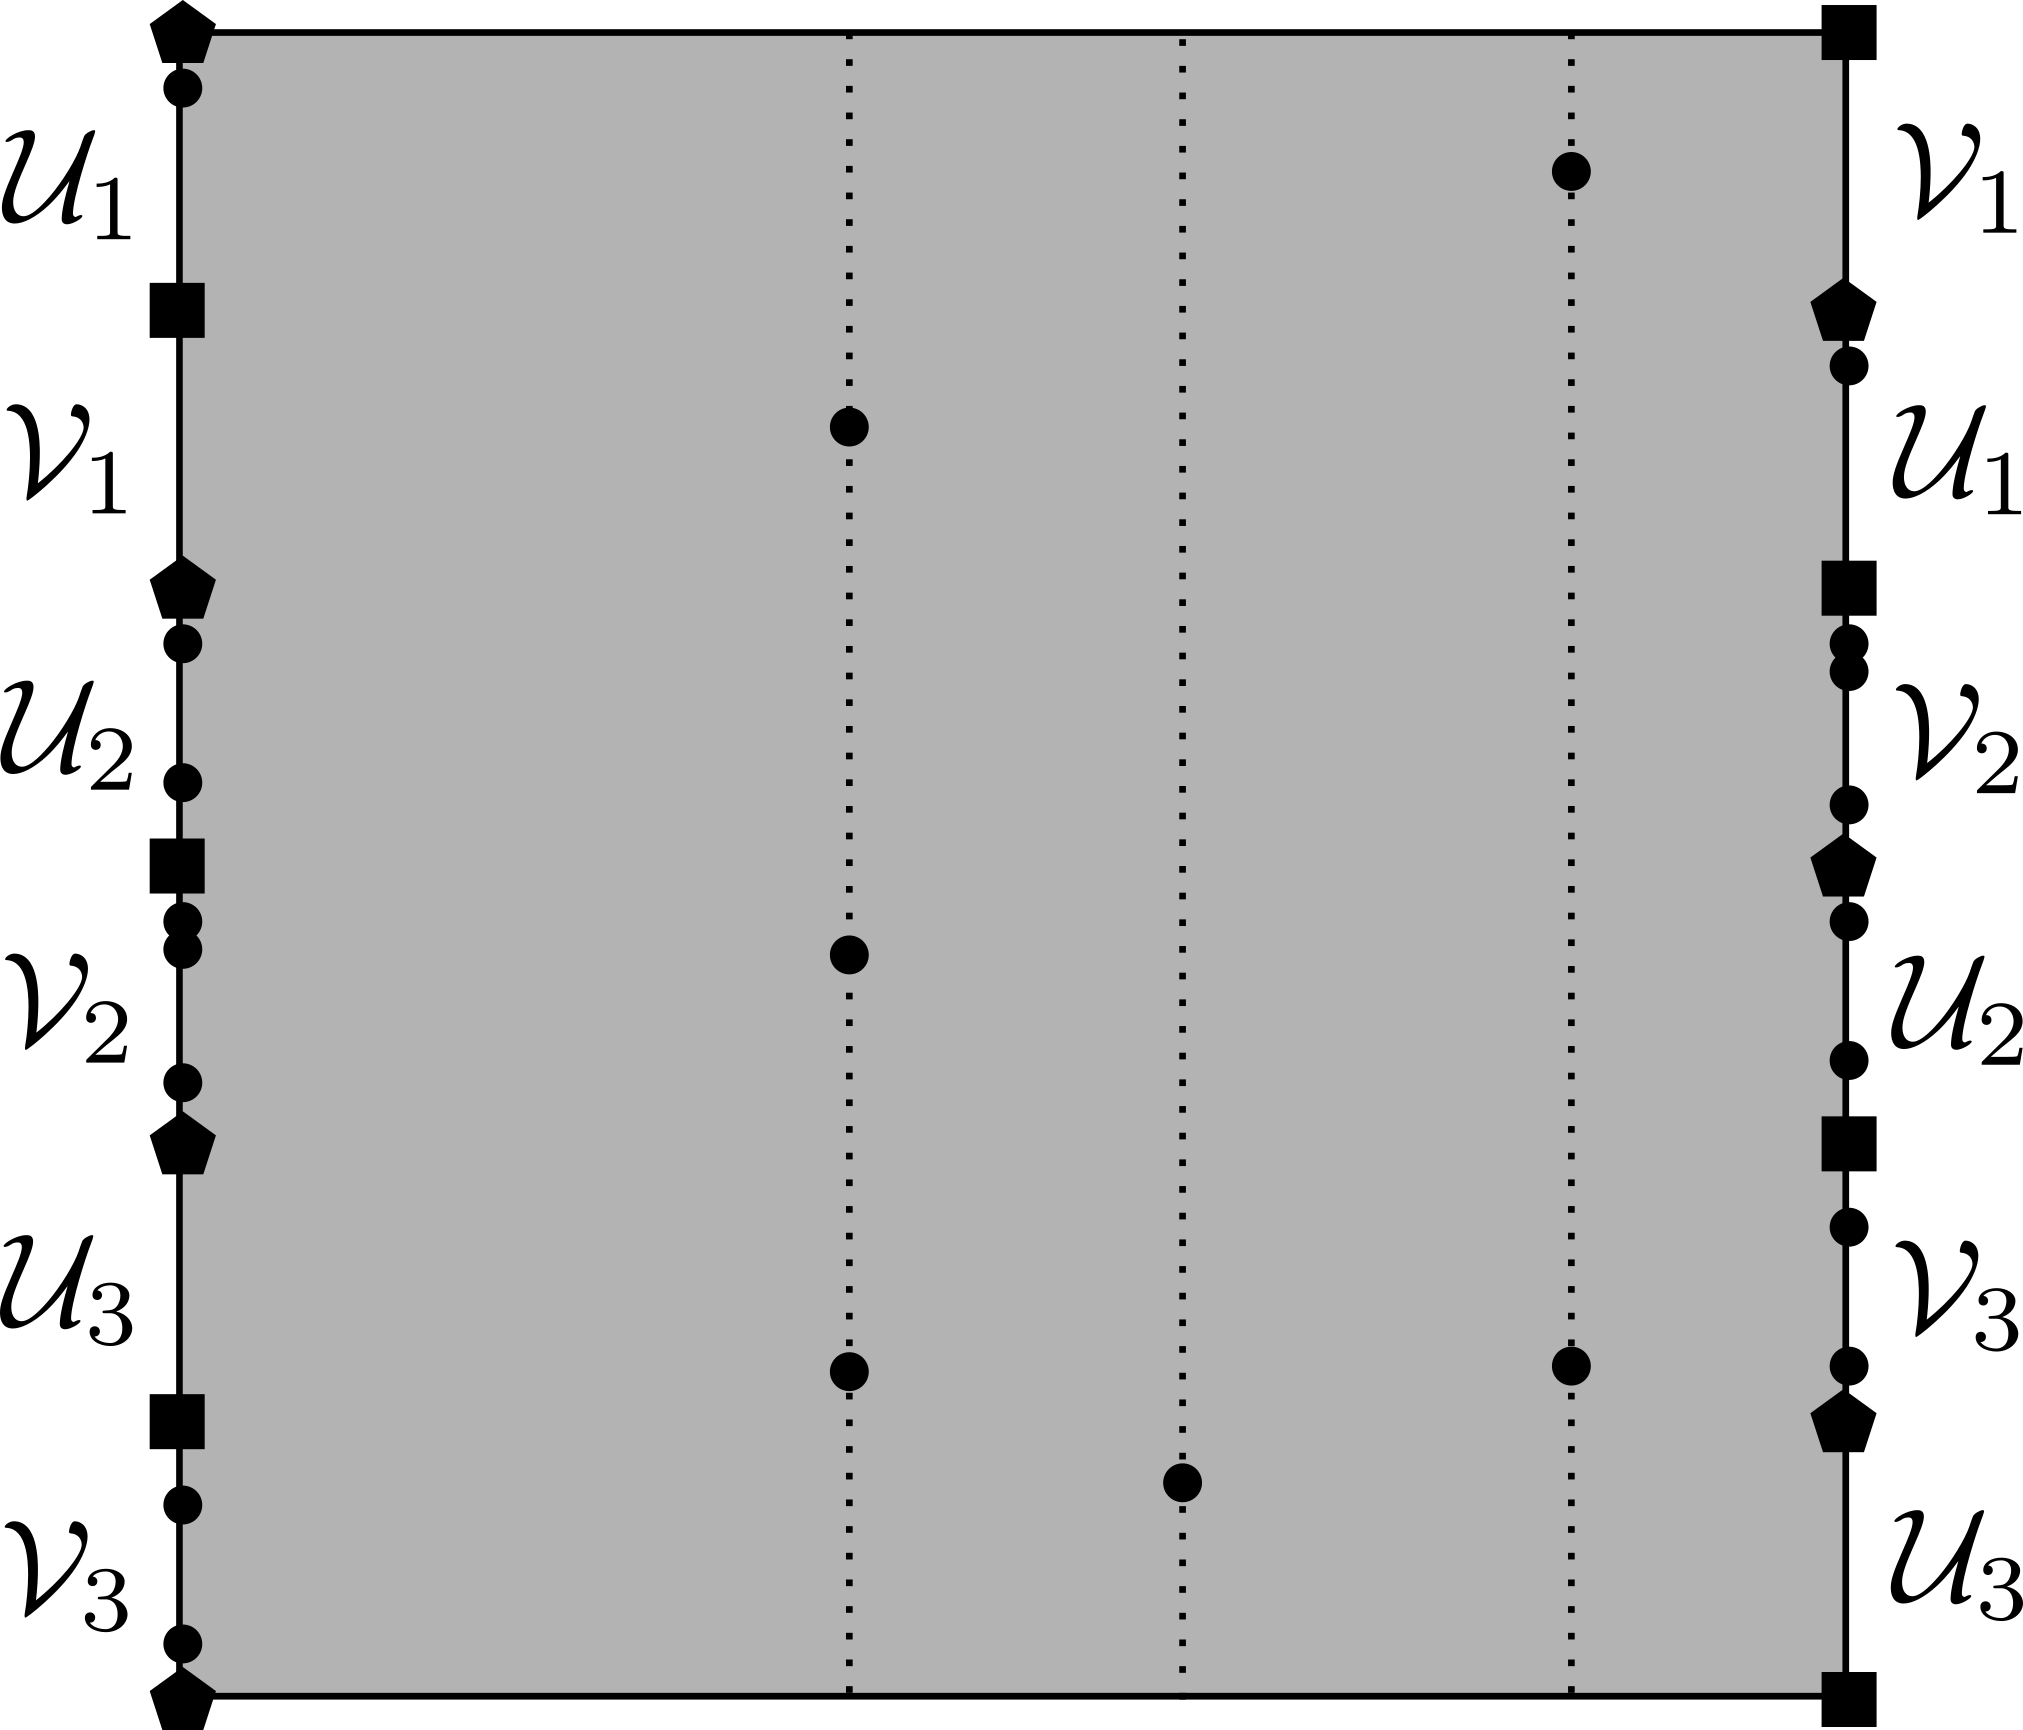
\includegraphics[scale=0.7]{figures/defetup.png}
 \caption{A configuration in the subspace $e^{\tup}\subset C_{14}(\S)$, for the tuple $\tup=(3,(3,1,2),(1,0,2,3,0,2))$. }
\label{fig:defetup}
\end{figure}


The space $e^{\tup}$ is homeomorphic to \emph{the interior} of the following product of simplices:

% We want to show that the collection of the $e_h$ for varying $h$, together with
% the 0-cell $*$, give a cell decomposition of $C_k(\S)^c$. Denote by $\Delta^h$ the following product of simplices
\[
 \Delta^{\tup}\colon =
 \Delta^l\times\prod_{i=1}^l\Delta^{x_i}\times\prod_{i=1}^g\pa{\Delta^{u_i}\times\Delta^{v_i}},
%  =\prod_{m\in\symb_l}\Delta^m.
\]
where the simplex $\Delta^r$ is the subspace of $[0,1]^r$ of sequences $0\leq \tau_1\leq\dots\leq\tau_r\leq 1$
(the numbers $\tau_1,\dots,\tau_r$ are the \emph{local coordinates} of the simplex). The homeomorphism is given
as follows:
\begin{itemize}
 \item the local coordinates of the $\Delta^l-$factor correspond to the positions $s_1,\dots,s_l$ of the vertical
 lines in $(0,1)^2$ containing points of the configuration;
 \item the local coordinates of the $\Delta^{x_i}-$factor correspond to the positions of the $x_i$ points
 lying on the vertical line $\set{s_i}\times(0,1)$;
 \item the local coordinates of the $\Delta^{u_i}-$factor correspond to the positions of the $u_i$ points
 lying on $\U_i$, which is canonically identified with $(0,1)$; similarly for the $\Delta^{v_i}-$factor,
 with $v_i$ and $\V_i$ instead of $u_i$ and $\U_i$.
\end{itemize}
Notice that the dimension of $\Delta^{\tup}$ is equal to the degree of $\tup$.
The embedding $\mathring{\Delta}^{\tup}\cong e^{\tup}\hookrightarrow \cms^c$ extends to a continuous map
$\phi^{\tup}\colon\Delta^{\tup}\to\cms^c$, so that the image of $\partial\Delta^{\tup}$ is contained in the union of
all subspaces $e^{\tup'}$ for tuples $\tup'$ with \emph{lower} degree than $\tup$, together with the point $\infty$.

The construction of the map $\phi^{\tup}$ is as follows:
\begin{enumerate}
\item we identify the one-point compactification
$(\mrS)^c$ of $\mrS=\T(\S)$ as the quotient of $[0,1]^2$ that identifies left and right intervals as in
in definition \ref{defn:Tsg} of $\T(\S)$, and moreover collapses $[0,1]^2\setminus Q$ to the point $\infty$;
\item we consider the $m-$fold symmetric product $\SP^m\pa{(\mrS)^c}$: it contains 
as an \emph{open} subspace $\cms$, so we can identify $\cms^c$ as the quotient of $\SP^m\pa{(\mrS)^c}$ collapsing
the subspace $\SP^m\pa{(\mrS)^c}\setminus\cms$ to $\infty$;
\item the homeomorphism $\mathring{\Delta}^{\tup}\to e^{\tup}\subset\cms$ extends
now to a map $\Delta^{\tup}\to\SP^m\pa{[0,1]^2}$, that we can then further project to
$ \SP^m\pa{(\mrS)^c}$ and then to $\cms^c$: the composition
is the map $\phi^{\tup}$.
\end{enumerate}

Therefore the collection of the $e^{\tup}$'s, together with the $0-$cell $\infty$,
gives a cell decomposition of $\cms^c$, with characteristic maps of cells $\phi^{\tup}$.

We can use these characteristic maps to compute the \emph{reduced} cellular chain complex of $\cms^c$
with coefficients in $\Z_2$, which
reads as follows.
\begin{lem}
\label{lem:doperatoropenmodtwo}
Let $\tup=(l,(x_i)_{i\leq l},(u_i,v_i)_{i\leq g})$ and
$\tup'=(l-1,(x'_i)_{i\leq l-1},(u'_i,v'_i)_{i\leq g})$
be tuples in consecutive degrees $m+l$ and $m+l-1$, and let $[\partial \tup\colon\tup']\in\Z_2$ denote the coefficient
of $\tup'$ in $\partial \tup$ in the reduced chain complex $\tilde\Ch_*(\cms^c)$.
Then $[\partial \tup:\tup']=0$ unless one (and exactly one) of the following situations occur:
\begin{itemize}
 \item $l\geq 2$ and $\tup'$ is obtained from $\tup$ by decreasing $l$ by 1, setting $x'_i=x_i+x_{i+1}$
 for one value $1\leq i\leq l-1$, and shifting the values
 $x'_j=x_{j+1}$ for $i+1\leq j\leq l-1$. We call this way to obtain $\tup'$ from $\tup$ an \emph{inner differential}.
 In this case
 \[
  [\partial \tup\colon\tup']=\binom{x_i+x_{i+1}}{x_i}.
 \]
 This binomial coefficient may be anyway equal to $0\in\Z_2$.
 \item $l\geq 1$ and $\tup'$ is obtained from $\tup$ by decreasing $l$ by 1, choosing a splitting of $x_1$
 in integers $\delta u_i,\delta v_i\geq 0$
 \[
  x_1=\sum_{i=1}^g \pa{\delta u_i+\delta v_i},
 \]
 setting $u'_i=u_i+\delta u_i$ and $v'_i=v_i+\delta v_i$ for all $1\leq i\leq g$ and shifting the values
 $x'_j=x_{j+1}$ for $1\leq j\leq l-1$. We call this a \emph{left, outer differential}. In this case
 \[
  [\partial \tup\colon\tup']=\prod_{i=1}^g\binom{u_i+\delta u_i}{u_i}\binom{v_i+\delta v_i}{v_i}.
 \]
 This product of binomial coefficients may be anyway equal to $0\in\Z_2$.
 \item $l\geq 1$ and $\tup'$ is obtained from $\tup$ by decreasing $l$ by 1, choosing a splitting of $x_l$
 in integers $\delta u_i,\delta v_i\geq 0$
 \[
  x_l=\sum_{i=1}^g \pa{\delta u_i+\delta v_i},
 \]
 setting $u'_i=u_i+\delta u_i$ and $v'_i=v_i+\delta v_i$ for all $1\leq i\leq g$ and keeping $x'_i=x_i$ for all $1\leq i\leq l-1$.
 We call this a \emph{right, outer differential}. Also in this case
 \[
  [\partial \tup\colon\tup']=\prod_{i=1}^g\binom{u_i+\delta u_i}{u_i}\binom{v_i+\delta v_i}{v_i}.
 \]
 This product of binomial coefficients may be anyway equal to $0\in\Z_2$.
\end{itemize}
\end{lem}
\begin{proof}
 If we restrict the map $\phi^{\tup}\colon\Delta^{\tup}\to\cms^c$ to any face of the multisimplex
 $\Delta^{\tup}$ coming from a factor different from $\Delta^l$,
 we obtain a constant map to $\infty$, hence these faces don't contribute
 to the boundary of $e^{\tup}$ in the reduced cellular chain complex. Instead for $0\leq i\leq l$ the restriction
 \[
  \phi^{\tup}\colon\partial_i\Delta^l\times\prod_{i=1}^l\Delta^{x_i}\times\prod_{i=1}^g\pa{\Delta^{u_i}\times\Delta^{v_i}}\to\cms^c
 \]
 hits homeomorphically the open cell $e^{\tup'}$
 exactly as many times as specified in the statement
 of the lemma for the cases $1\leq i\leq l-1$,
 $i=0$ and $i=l$ respectively, and no other open cell of dimension $m+l-1$.
 We are working in $\Z_2$ so we don't have to be careful about orientations of cells
 and therefore about signs.
\end{proof}

We can filter the chain complex $\tilde\Ch_*(\cms^c)$ by giving norm $\sum_{i=1}^lx_i$ to
the cell $e^{\tup}$, with $\tup=(l,(x_i)_{i\leq l},(u_i,v_i)_{i\leq g})$; for example
the cell in figure \ref{fig:defetup} has norm 6. By lemma \ref{lem:doperatoropenmodtwo}
the norm is weakly decreasing along differentials. Let $F_p\subset\tCh_*(\cms^c)$ be the subcomplex of cells
of norm $\leq p$, and let $F_p/F_{p-1}$ be the $p-$th filtration stratum.

Then $F_p/F_{p-1}$ is isomorphic, as a chain complex, to a direct sum of copies of $\tCh_*(C_p(\Sigma_{0,1}))$,
one copy for each way of splitting $(m-p)=\sum_{i=1}^g (u_i+v_i)$ with $u_i,v_i\geq 0$. The isomorphism
doesn't preserve the degrees but shifts them by $p$.

Indeed in $F_p/F_{p-1}$ all outer
differentials vanish (see lemma \ref{lem:doperatoropenmodtwo}
for the definition), and in particular the numbers $u_i,v_i$
don't change along the differentials of $F_p/F_{p-1}$. Therefore $F_p/F_{p-1}$ splits as a direct sum
of chain complexes indexed by splittings $(m-p)=\sum_{i=1}^g (u_i+v_i)$ as above.
It is then immediate to identify the inner differentials
with the ones one would have in the case $g=0$, i.e. for the surface $\Sigma_{0,1}$.

We notice that $\tCh_*(C_p(\Sigma_{0,1})^c)$ is exactly the chain complex described by Fuchs in
\cite{Fuchs:CohomBraidModtwo}, so we pause for a moment and
recall some classical facts about the cohomology of configuration
spaces of the disc.
\begin{defn}
\label{defn:symchain}
Given a splitting $p=\sum_{j=0}^{\infty}\alpha_j2^j$ of $p$ into powers of 2, with multiplicities $\alpha_j$,
the associated \emph{symmetric chain} in $\tCh_*(C_p(\Sigma_{0,1})^c)$
is the sum of all $e^{\tup}$ where $\tup$ ranges among all tuples
$\pa{l,(x_i)_{i\leq l}}$ such that
\begin{itemize}
 \item $l=\sum_{j=1}^{\infty}\alpha_j$;
 \item every $x_i$ is a power of 2;
 \item for all $j\geq 0$ there are exactly $\alpha_j$ indices $i$ such that $x_i=2^j$.
\end{itemize}
Here and in the following it is understood that $\alpha_j=0$ for all but finitely many indices $j$.

We denote by $|(\alpha_j)_{j\geq 0}|\in\tCh_{p+l}(C_p(\Sigma_{0,1})^c)$ the symmetric chain
and by $[(\alpha_j)_{j\geq 0}]\in\tH_{p+l}(C_p(\Sigma_{0,1})^c)$ the associated homology class.
\end{defn}
In \cite{Fuchs:CohomBraidModtwo} Fuchs shows that a graded basis for $\tH_*(C_p(\Sigma_{0,1})^c)$
is given by the collection of all classes $[(\alpha_j)_{j\geq 0}]$ satisfying $p=\sum\alpha_j2^j$.

By Poincaré-Lefschetz duality this is a basis for the cohomology $H^*(C_p(\Sigma_{0,1}))$.
The \emph{dual} basis of $H_*(C_p(\Sigma_{0,1}))$
happens to be the basis of monomials
$\prod_{j\geq 0}(Q^i\epsilon)^{\alpha_j}\in H_*(C_p(\Sigma_{0,1}))$, that is, all monomials
of weight $p$, using
the isomorphism \ref{eq:Cohen} in its full meaning (i.e. as an isomorphism of rings,
where $Q$ denotes the first Dyer-Lashof operation).

% This notation is compatible, after interpreting equation \ref{eq:genuszero} as an isomorphism
% of rings, with the results of \cite[Chap.3]{CLM}: the monomials constructed there, using
% the Pontryagin product and the operation $Q$, are really the dual basis of the basis of
% symmetric chains for cohomology.

We will not need this finer result in this article, so in the following the expression
$\prod_{j\geq 0}(Q^i\epsilon)^{\alpha_j}\in H_{p-l}(C_p(\Sigma_{0,1}))$ will only denote
the (unique) homology class whose algebraic intersection with $[(\alpha'_j)]\in\tH_{p+l}(C_p(\Sigma_{0,1})^c)$
is $1\in\Z_2$ if and only if the equality $\alpha_j=\alpha'_j$ holds for all $j\geq 0$.
% i.e. we \emph{define} monomials as the dual basis of the basis of symmetric chains, and keep considering
% \ref{eq:Cohen} only as an isomorphism of bigraded vector spaces.

We now go back to the filtered chain complex $\tCh_*(\cms^c)$:
if we run the associated Leray spectral sequence,
the $E^1-$page contains on the $p-$th column the homology of $F_p/F_{p-1}$; as we have seen this consists of
many copies of the homology of $\tCh_*(C_p(\Sigma_{0,1}))$, each generated by symmetric chains.

\begin{defn}
\label{defn:gensymchain}
For a splitting
\[
 m=p+(m-p)=\pa{\sum_{j=0}^{\infty}\alpha_j2^j}+\pa{\sum_{i=1}^g(u_i+v_i)}
\]
let $l=\sum_{j=1}^{\infty}\alpha_j$. We define a chain in
$\tCh_{m+l}(\cms)$, denoted by $|p,(\alpha_j)_j,(u_i,v_i)_{i\leq g}|$: it
is obtained by summing all $e^{\tup}$ where $\tup$
ranges among all tuples of the form $\pa{l,(x_i)_{i\leq l},(u_i,v_i)_{i\leq g}}$
satisfying the three properties listed in definition \ref{defn:symchain}.

We call such a chain a
\emph{generalised symmetric chain}, and its homology class in $\tH_{m+l}(\cms^c)$ is denoted
by $[p,(\alpha_j),(u_i,v_i)]$
\end{defn}

We notice now that a generalised symmetric chain $|p,(\alpha_j),(u_i,v_i)|$
is not only
a cycle when projected to its filtration quotient $F_p/F_{p-1}$, as the $E^1-$page
of the spectral sequence tells us, but also
in the chain complex $\tCh_*(\cms^c)$ itself. Indeed also all outer
differentials of a generalised symmetric chain cancel out: in particular
every left differential
of one cell $e^{\tup}$ in the generalised symmetric chain cancels out with a right differential
of possibly another cell $e^{\tup'}$.

Therefore the spectral sequence collapses on its first page and
% $H_*(\cms^c)$
% has a $\Z_2$-basis given by generalised symmetric chains.
we have the following lemma:
\begin{lem}
\label{lem:gensymchain}
The homology $H_*(\cms^c)$ has a graded basis given by the classes $[p,(\alpha_j),(u_i,v_i)]$
associated to generalised symmetric chains of weight $m$.
% this basis is bijection with
% the choices of the following set of data:
% \begin{itemize}
%  \item a number $0\leq p\leq m$;
%  \item a splitting $m-p=\sum_{i=1}^g (u_i+v_i)$ with $u_i,v_i\geq 0$;
%  \item a splitting $p=\sum_{j=0}^{\infty}\alpha_j2^j$ with $\alpha_j\geq 0$.
% \end{itemize}
% The homology class $[p,(u_i,v_i),(\alpha_j)]\in H_*(\cms^c)$ has homological degree
% $m+\sum_{j=1}^{\infty}\alpha_j$.
\end{lem}
% To interpret this class
% as a monomial in the tensor product of theorem \ref{thm:Hbms*as*ggrep} we need the following definition.

% We are almost ready to prove an isomorphism of bigraded $\Z_2-$vector spaces as in theorem \ref{thm:Hbms*as*ggrep}.

\begin{defn}
 \label{defn:dualHbasis}
We can see the $\U_i$'s and $\V_i$'s as properly embedaded $1-$manifolds in $\mrS$;
by Poincaré-Lefschetz duality they represent classes in $\tH_1\pa{(\mrS)^c}\simeq H^1(\S)$,
and in particular they form a basis
of the latter cohomology group. We call $\u_i,\v_i\in H_1\pa{\mrS}$ the dual basis.

% We fix simple closed curves $\u_i,\v_i$ on $\S$, for $1\leq i\leq g$, whose fundamental classes
% $[\u_i],[\v_i]$ form the dual basis of $H_1(\S)$. We assume that, apart from the following necessary exceptions,
% all curves $\U_i,\V_i,\u_i,\v_i$ for $1\leq i\leq g$ are disjoint:
% \begin{itemize}
%  \item $\u_i$ and $\v_i$ intersect once, transversely;
%  \item $\u_i$ and $\U_i$ intersect once, transversely;
%  \item $\v_i$ and $\V_i$ intersect once, transversely;
%  \end{itemize}
% SEE PICTURE.
\end{defn}
We establish a bijection between monomials in the tensor product of theorem  \ref{thm:Hbms*as*ggrep}
and the basis of $H^*(\cms)\simeq H_*(\cms^c)$ in lemma \ref{lem:gensymchain}:
the class 
\[
[p,(u_i,v_i),(\alpha_j)]\in H_{m+\sum\alpha_j}(\cms^c)\simeq H^{m-\sum\alpha_j}(\cms)
\]
is associated with the monomial $\prod_{j=1}^{\infty}(Q^j\epsilon)^{\alpha_j}\otimes \prod_{i=1}^g([\u_i]^{u_i}[\v_i]^{v_i})$.

This shows an isomorphism of bigraded $\Z_2-$vector spaces
\begin{equation}\label{eq:isovectorspaces}
  \bigoplus_{m\geq 0} H^*(\cms)\simeq \Z_2\left[Q^j\epsilon\,|\, j\geq 0\right]\otimes\Sym_{\bullet}(\H),
\end{equation}
from which we conclude that
there exists an isomorphism as in theorem \ref{thm:Hbms*as*ggrep}
at least \emph{as bigraded $\Z_2-$vector spaces}: the two bigraded
vector spaces have the same dimension in all bidegrees.